\documentclass[12pt,a4paper]{ctexart}

\usepackage{geometry}
\usepackage{graphicx}
\usepackage{amsmath}
\usepackage{amssymb}
\usepackage{array}
\usepackage{booktabs}
\usepackage{xeCJK}
\usepackage{tikz}
\usepackage{titlesec}

% 页面设置
\geometry{
    top=2.5cm,
    bottom=2.5cm,
    left=2.8cm,
    right=2.8cm
}

% 定义 section* 格式
\titleformat{\section}
  {\zihao{-3}\heiti\bfseries}
  {}
  {0em}
  {}
\titlespacing*{\section}{0pt}{0.5cm}{0.3cm}  % 左缩进、上间距、下间距


% 取消页码（封面）
\pagestyle{empty}

% 定义等长下划线命令（固定宽度 6.5cm，左对齐）
\newcommand{\infofill}[1]{{\zihao{4}\songti\underline{\makebox[6.5cm][c]{#1}}}}

% 定义内容区块命令
\newcommand{\reportsection}[2]{%
    \noindent{\zihao{-3}\heiti\bfseries #1（#2分）}
    \vspace{0.3cm}
    
    \noindent\rule{\textwidth}{0.4pt}
    \vspace{6cm}
}

% 设置中文字体
\setCJKmainfont{SimSun}  % 宋体，可根据系统改为 Noto Serif CJK SC 等

\begin{document}
% ==================== 封面页 ====================
\begin{titlepage}
    \centering
    \vspace*{1.5cm}
    % 校徽占位（正方形示例图）
    
\includegraphics[width=5cm,height=5cm]{images/image-2026-09-07-14-57-04.png}
    
    \vspace{1.8cm}
    
    % 中山大学
    {\zihao{1}\heiti\bfseries 中山大学}
    
    \vspace{0.9cm}
    
    % 微电子科学与技术学院
    {\zihao{2}\heiti 微电子科学与技术学院}
    
    \vspace{0.9cm}
    
    % 课程名称
    {\zihao{2}\heiti 《集成电路元器件特性表征实验》}
    
    \vspace{0.9cm}
    
    % 实验报告
    {\zihao{1}\heiti\bfseries 实验报告}
    
    \vspace{3cm}
    
    % 信息表格
    

    % 信息表格（无任何框线，无横线，无竖线）
    \begin{tabular}{@{}>{\zihao{4}\heiti}r @{\hspace{1.2em}} l@{}}
        实验主题      & \infofill{光电导衰减法测量硅电池少子寿命}        \\[0.8cm]
        姓\quad\quad 名 & \infofill{徐睿琳}   \\[0.8cm]
        学\quad\quad 号 & \infofill{23342107} \\[0.8cm]
        实验日期      & \infofill{\today}   \\[0.8cm]
    \end{tabular}
    
    \vfill
\end{titlepage}

% ==================== 内容页 ====================
\newpage
\pagestyle{plain}
\setcounter{page}{2}

\section*{实验目的（5分）}
\begin{enumerate}
    \item 明确非平衡少数载流子的定义，理解少子寿命的物理意义及其对半导体器件性能的影响。
    \item 掌握高频光电导衰减法测量硅电池少子寿命的原理与实验方法。
    \item 通过指数衰减曲线拟合求得少子寿命 $\tau$，并研究光源驱动频率对测量结果的影响。
\end{enumerate}

\section*{实验原理（10分）}

\subsection*{1. 非平衡载流子与少子寿命}
在非平衡状态下，半导体中载流子浓度偏离热平衡值，超出部分称为非平衡载流子，记为 $\Delta n$、$\Delta p$。光照停止后，非平衡载流子通过复合逐渐消失，其平均生存时间定义为少数载流子寿命 $\tau$。少子寿命是表征晶体结构完整性与深能级杂质含量的重要参数，直接影响太阳电池转换效率、双极器件电流增益与开关速度等性能。

\subsection*{2. 光电导效应}
无光照时半导体电导率为
\begin{equation}
    \sigma_0 = q(n_0\mu_n + p_0\mu_p),
\end{equation}
其中 $q$ 为元电荷，$\mu_n$、$\mu_p$ 分别为电子与空穴迁移率。脉冲光照射产生非平衡载流子 $\Delta n = \Delta p$，引起附加光电导
\begin{equation}
    \Delta\sigma = q(\mu_n + \mu_p)\Delta n,
\end{equation}
样品电阻随之下降，测试回路电流幅值相应增加 $\Delta I$。

\subsection*{3. 指数衰减规律}
光照消失后，非平衡载流子浓度按指数规律衰减：
\begin{equation}
    \Delta n(t) = \Delta n_0 e^{-t/\tau},
\end{equation}
附加光电导及回路电流同步衰减，其衰减速率由载流子在晶体内的平均存在时间决定。

\subsection*{4. 高频恒压测量与寿命提取}
高频源为恒压输出，样品电阻减小使流经样品的高频电流幅值增加 $\Delta I$，在取样电阻 $R$ 两端产生电压信号 $\Delta V = \Delta I R$。小注入条件下，当光照区载流子复合占主导时，$\Delta V$ 与 $\Delta n(t)$ 遵循同一衰减规律：
\begin{equation}
    \Delta V(t) = \Delta V_0 e^{-t/\tau}.
    \label{eq:decay}
\end{equation}
用示波器记录光照停止后 $\Delta V$ 随时间的衰减曲线，按式 \eqref{eq:decay} 拟合即得少子寿命 $\tau$。

\subsection*{5. 有效寿命}
若样品同时存在体内复合与表面复合，测得的有效寿命满足
\begin{equation}
    \frac{1}{\tau_{\mathrm{eff}}} = \frac{1}{\tau_b} + \frac{1}{\tau_s},
\end{equation}
其中 $\tau_b$ 为体内寿命，$\tau_s$ 为表面复合贡献的等效寿命。

本方法属瞬态法（直接法），样品无需切割成形、无须制作欧姆电极，故污染少、操作简便，为国际上通用的少子寿命测量方法。

\section*{实验设备和步骤（5分）}

\subsection*{实验设备}
信号发生器 1 台、示波器 1 台、发光二极管（LED）1 个、硅电池（光电探测器）1 个、取样电阻 $R$、导线若干。测试电路如图 6.1 所示，高频源、样品与取样电阻串联，LED 由信号发生器驱动的方波信号调制，硅电池输出信号送入示波器。

\subsection*{实验步骤}
\begin{enumerate}
    \item 用导线正确连接信号发生器与示波器，按图 6.1 将发光二极管与硅电池接入测试电路，注意正负极不得接反。
    \item 接通示波器与信号发生器电源，设置信号发生器输出方波：幅值 $10\ \mathrm{V}$、频率 $400\ \mathrm{Hz}$，使 LED 达到稳定亮度。
    \item 将 LED 贴近硅电池探头，调节示波器至显示清晰的衰减波形与读数。
    \item 采集光照停止后的 $\Delta V$--$t$ 衰减数据，按式 \eqref{eq:decay} 拟合，计算少子寿命 $\tau$。
    \item 依次设置驱动频率为 $200$、$400$、$600$、$800$、$1000\ \mathrm{Hz}$，重复上述测量，研究驱动频率对少子寿命测量结果的影响。
\end{enumerate}

\section*{实验数据分析（50分）}

\subsection*{1. 数据预处理}
示波器原始记录每频点 $10^6$ 点，采样率为 $10$ MSa/s（$200$、$400$ Hz）或 $100$ MSa/s（$600$、$800$、$1000$ Hz），覆盖 $4\sim8$ 个完整调制周期。单点噪声与量化台阶（$0.44$~mV）与信号幅度（约 $20$~mV）同量级，故先作周期折叠平均：以驱动周期 $T=1/f$ 为窗，按相位对齐后逐点平均，等效平均 $4\sim8$ 个周期，有效信噪比提升 $\sqrt{N}$ 倍以上。

\subsection*{2. 波形结构与衰减区间识别}
以标准条件 $400$~Hz 为例，单周期波形如图 \ref{fig:waveform} 所示。方波调制下波形由两种过程叠加：开灯沿存在时间尺度 $<10~\mu$s、幅度约 $11$~mV 的快速跳变，源于驱动方波边沿经寄生耦合进入测量回路，属电路瞬态，不反映载流子复合；开灯后与关灯后的慢过程（时间尺度数百 $\mu$s）则反映非平衡载流子的积累与复合。关灯后电压由饱和值 $V_{\mathrm{light}}$ 平滑弛豫至暗态 $V_{\mathrm{dark}}$，衰减段不含快成分，符合式 \eqref{eq:decay}，故取关灯沿至下一开灯沿之间的数据段进行拟合。

具体处理：以折叠波形梯度最大值定位开灯瞬变沿，按 $50\%$ 占空比取关灯沿（相位相差 $T/2$）；以开灯沿前 $60~\mu$s 内电平的中位数为暗态基线 $V_{\mathrm{dark}}$，关灯后 $2~\mu$s 内电平为 $V_{\mathrm{light}}$，令 $\Delta V(t)=V(t)-V_{\mathrm{dark}}$。

\subsection*{3. 指数拟合与少子寿命}
按式 \eqref{eq:decay} 对 $\Delta V$--$t$ 作非线性最小二乘拟合，拟合区间取幅度衰减至初始值 $10\%$（约 $2.3\tau$）处，高频下半周期不足时截断至半周期末端；同时给出 $\tau_{1/e}$（$\Delta V$ 衰减至 $\Delta V_0/e$ 的时间）作交叉验证。$400$~Hz 的拟合结果如图 \ref{fig:decay} 所示，各频点结果列于表 \ref{tab:tau}。

\begin{table}[htbp]
\centering\small
\caption{不同驱动频率下的光电导衰减拟合结果}
\label{tab:tau}
\begin{tabular}{ccccccccc}
\toprule
$f$ (Hz) & $T/2$ ($\mu$s) & $N$ & $V_{\mathrm{dark}}$ (mV) & $\Delta V_0$ (mV) & $\tau$ ($\mu$s) & $\tau_{1/e}$ ($\mu$s) & $\sigma_\tau$ ($\mu$s) & $R^2$\\
\midrule
200  & 2500 & 4 & $-18.58$ & $-19.05$ & 481.7 & 500.2 & 20.4 & 0.9946\\
400  & 1250 & 8 & $-22.59$ & $-22.67$ & 425.6 & 451.9 & 5.6  & 0.9920\\
600  & 833  & 6 & $-25.47$ & $-19.66$ & 347.5 & 372.8 & 4.1  & 0.9860\\
800  & 625  & 4 & $-26.59$ & $-14.73$ & 274.9 & 291.8 & 6.5  & 0.9845\\
1000 & 500  & 5 & $-29.26$ & $-13.91$ & 235.2 & 252.6 & 6.0  & 0.9793\\
\bottomrule
\end{tabular}
\end{table}

\subsection*{4. 驱动频率对测量结果的影响}
由图 \ref{fig:compare}--\ref{fig:ampf} 可见，$\tau$ 与调制幅度 $|\Delta V_0|$ 均随 $f$ 单调下降。其物理原因在于：当半周期 $T/2$ 与 $\tau$ 可比时，非平衡载流子在一个半周期内既未能积累至稳态 $\Delta n_{ss}=G\tau$，又未能充分复合，衰减起点与基线均偏离稳态值，使按单指数定义的视在寿命被系统性低估；同时频率升高导致平均注入水平改变，而寿命本身具有注入水平依赖性。

以 $T/2\gtrsim5\tau$ 为充分衰减判据：$200$~Hz 时 $T/2=2500~\mu$s$\approx5.2\tau$，结果趋于稳定，可视为材料本征值；$1000$~Hz 时 $T/2=500~\mu$s$\approx2.1\tau$，衰减未完成，$\tau$ 被低估约 $51\%$。故本样品少子寿命取低频极限 $\tau\approx4.8\times10^{2}~\mu$s（$\approx0.48$~ms），标准条件 $400$~Hz 下 $\tau\approx4.3\times10^{2}~\mu$s。

\begin{figure}[htbp]
\centering
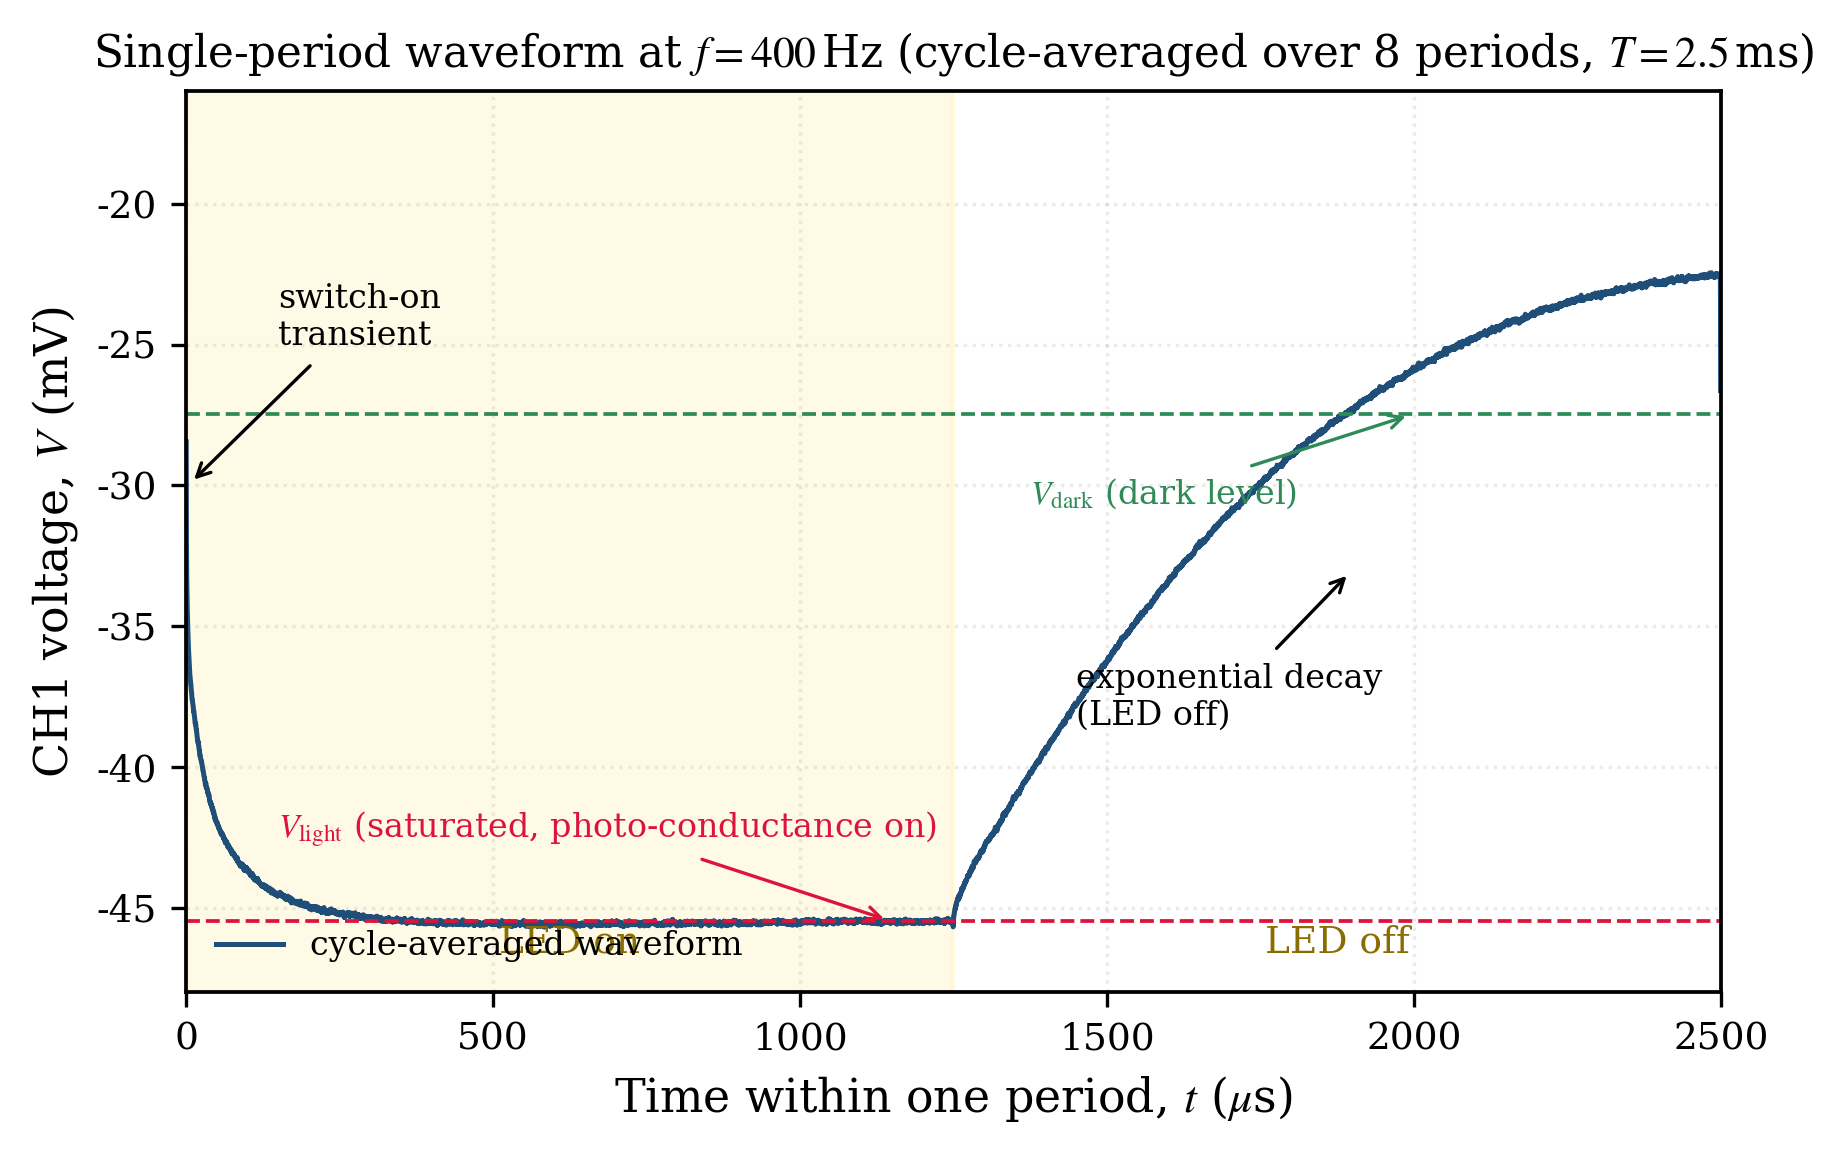
\includegraphics[width=0.82\textwidth]{images/image-2026-10-25-19-37-46.png}
\caption{$400$~Hz 下单周期折叠平均波形（$T=2.5$~ms）。}
\label{fig:waveform}
\end{figure}

\begin{figure}[htbp]
\centering
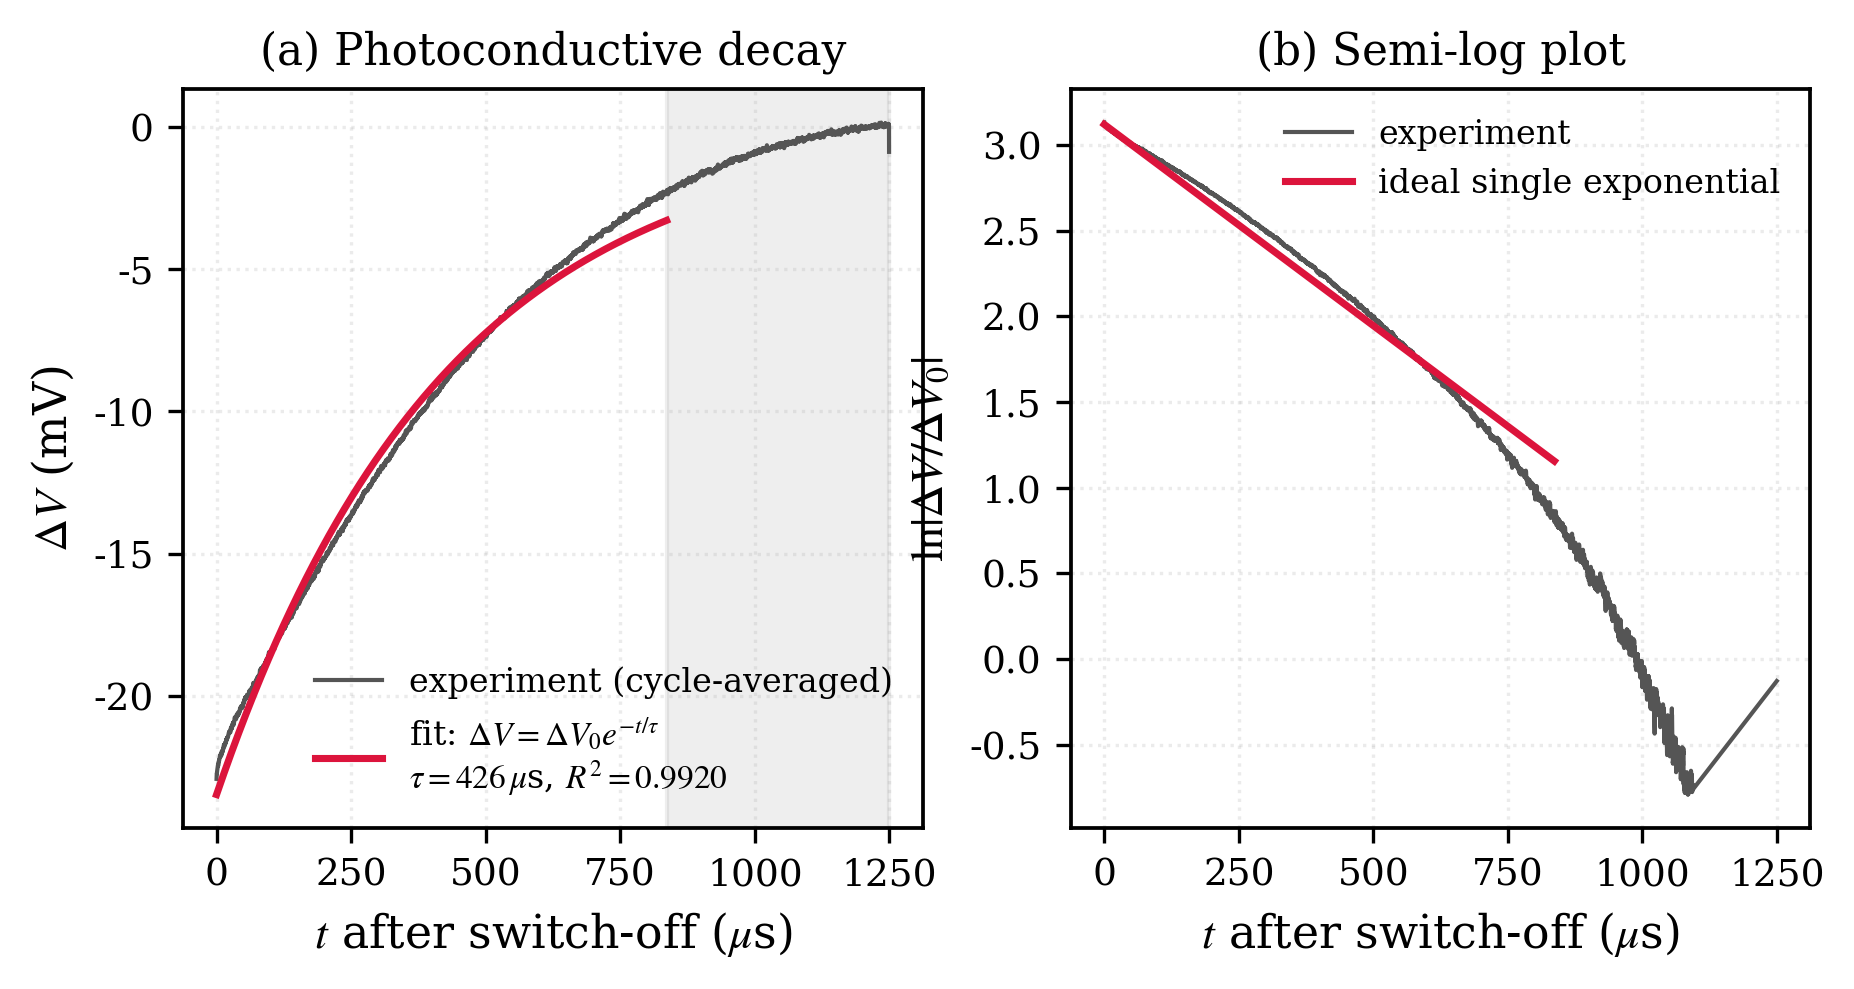
\includegraphics[width=0.95\textwidth]{images/image-2026-10-25-19-38-16.png}
\caption{$400$~Hz 关灯后光电导衰减曲线：(a) 线性坐标拟合；(b) 半对数坐标检验指数性。}
\label{fig:decay}
\end{figure}

\begin{figure}[htbp]
\centering
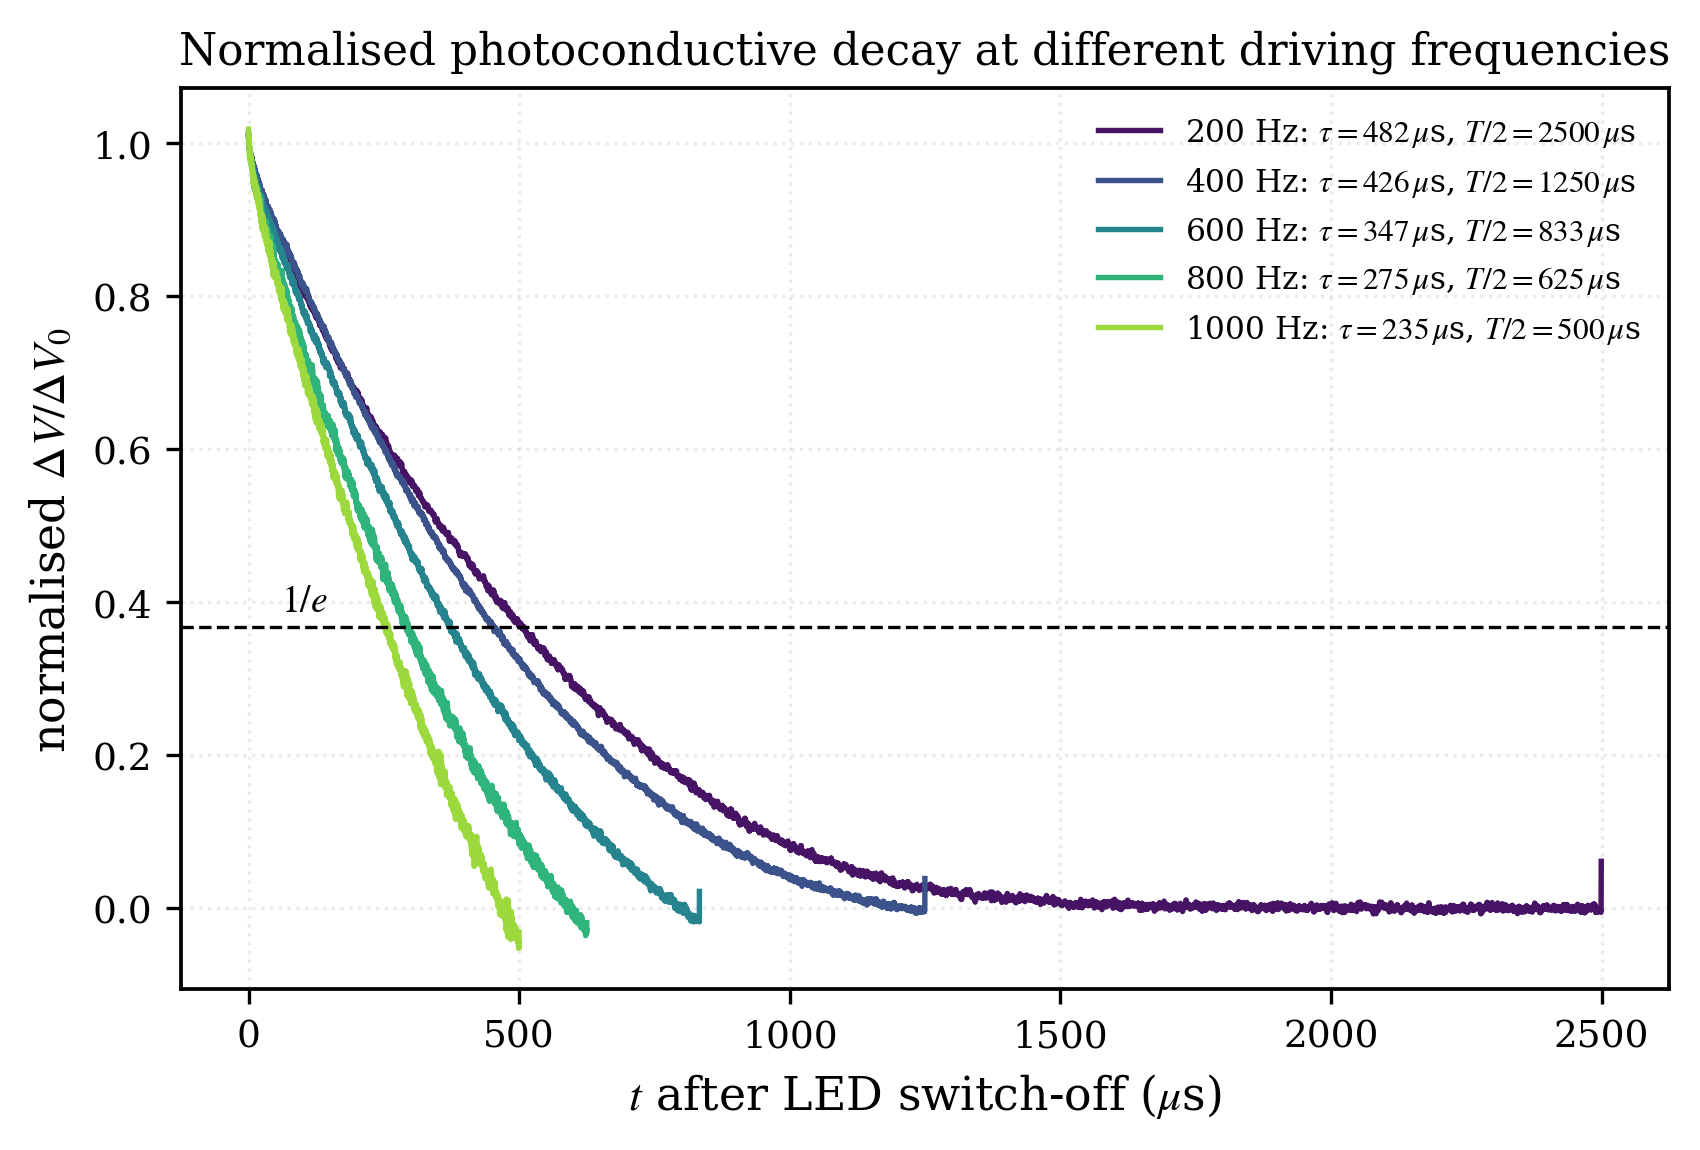
\includegraphics[width=0.82\textwidth]{images/image-2026-10-25-19-39-10.png}
\caption{不同驱动频率下归一化衰减曲线对比。}
\label{fig:compare}
\end{figure}

\begin{figure}[htbp]
\centering
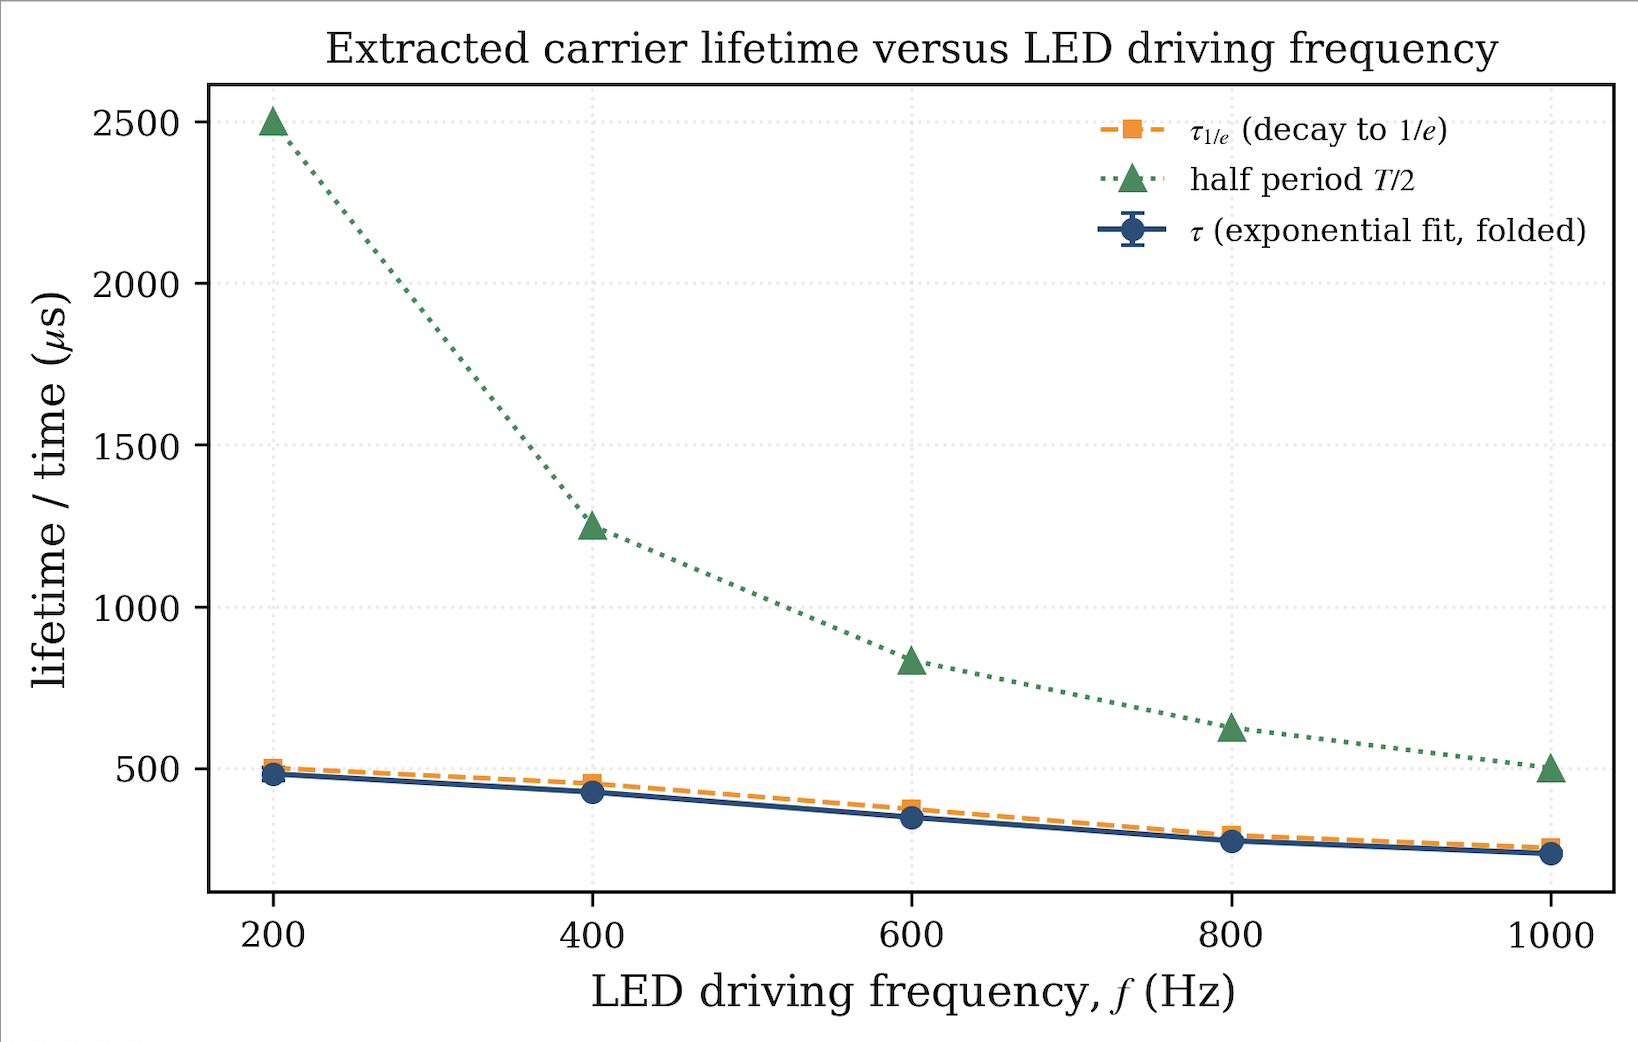
\includegraphics[width=0.82\textwidth]{images/image-2026-10-25-19-42-15.png}
\caption{提取寿命随驱动频率的变化（误差棒为周期间拟合标准差）。}
\label{fig:tauf}
\end{figure}

\begin{figure}[htbp]
\centering
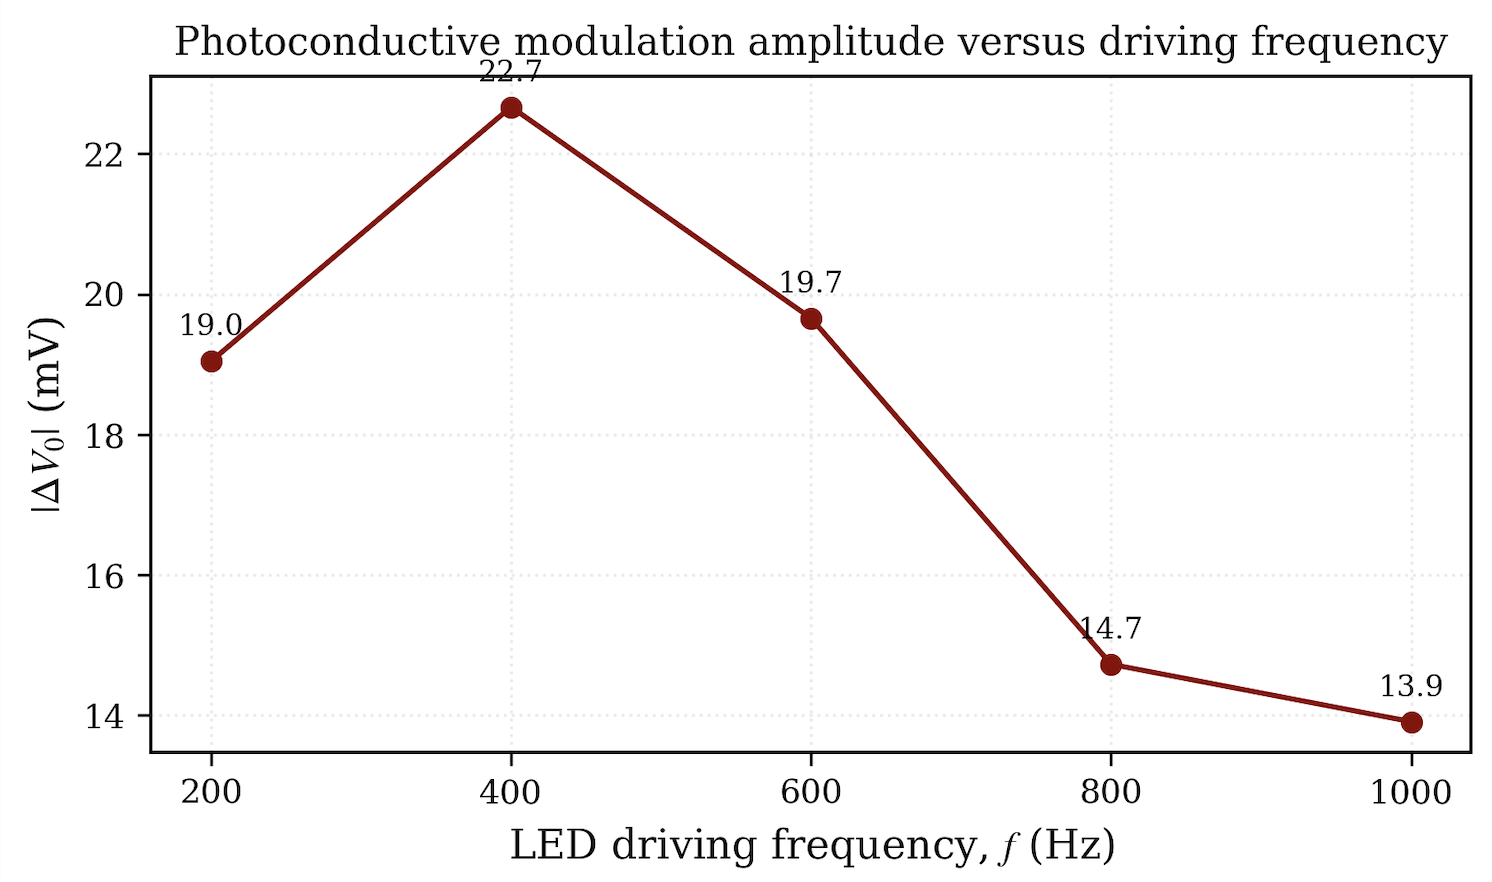
\includegraphics[width=0.82\textwidth]{images/image-2026-10-25-19-42-43.png}
\caption{光电导调制幅度随驱动频率的变化。}
\label{fig:ampf}
\end{figure}

\subsection*{5. 误差分析与讨论}
周期间独立拟合给出的标准差 $\sigma_\tau$ 为 $4.1\sim20.4~\mu$s（相对偏差 $<5\%$），表明测量重复性良好；$200$~Hz 因仅 $4$ 个周期且单点噪声较大，离散度相对较高。各频点 $R^2=0.979\sim0.995$，衰减主体符合单指数规律。半对数图（图 \ref{fig:decay}(b)）显示衰减尾部略偏离直线，提示存在少量慢复合通道（表面态或陷阱辅助复合），使全区间单指数拟合较 $\tau_{1/e}$ 低 $5\%\sim10\%$。此外样品未作表面钝化，按 $1/\tau_{\mathrm{eff}}=1/\tau_b+1/\tau_s$，所测为包含表面复合贡献的有效寿命，故 $\tau_{\mathrm{eff}}\leq\tau_b$。

\subsection*{6. 结论}
高频光电导衰减法测得该硅电池样品的非平衡少子寿命为 $\tau\approx0.48$~ms（$200$~Hz，低频极限），标准条件 $400$~Hz 下为 $0.43$~ms；驱动频率由 $200$~Hz 升至 $1000$~Hz 时，视在寿命由 $482~\mu$s 降至 $235~\mu$s，证实测量须满足 $T/2\gg\tau$ 方能获得可靠的少子寿命。

\section*{实验结论（20分）}

\begin{enumerate}
    \item \textbf{测量方法成立。}关灯后取样电阻两端电压 $\Delta V$ 的衰减主体严格遵循 $\Delta V=\Delta V_0e^{-t/\tau}$，各频点拟合 $R^2=0.979\sim0.995$，周期间重复拟合标准差 $<5\%$，证明在高频恒压条件下 $\Delta V\propto\Delta I\propto\Delta n$，由电压衰减直接提取少子寿命的方案可行。

    \item \textbf{样品少子寿命。}低频极限（$200$~Hz，$T/2\approx5.2\tau$）测得该硅电池样品非平衡少子寿命 $\tau\approx4.8\times10^{2}~\mu$s（$\approx0.48$~ms）；标准条件 $400$~Hz 下 $\tau\approx4.3\times10^{2}~\mu$s。该量级与太阳电池级单晶硅材料的典型值相符，表明样品晶体完整性较好、深能级复合中心浓度较低。

    \item \textbf{驱动频率的显著影响。}驱动频率由 $200$~Hz 升至 $1000$~Hz，视在寿命由 $482~\mu$s 单调降至 $235~\mu$s（低估约 $51\%$），光电导调制幅度同步由 $19.05$~mV 降至 $13.91$~mV（降幅 $27\%$）。根源在于 $T/2$ 与 $\tau$ 可比时，非平衡载流子既未积累至稳态 $\Delta n_{ss}=G\tau$，又未在一个半周期内充分复合，衰减起点与基线同时偏离稳态值，使单指数拟合给出的视在寿命被系统性低估。实验表明测量须满足 $T/2\gtrsim5\tau$ 才可获得逼近本征值的结果，这也即是思考题（1）的答案：LED 频率过高将严重低估少子寿命。

    \item \textbf{波形中的非复合成分须剔除。}开灯沿存在时间尺度 $<10~\mu$s、幅度约 $11$~mV 的快速跳变，系驱动方波边沿经寄生耦合进入测量回路所致，不代表载流子复合。若将其纳入拟合，会引入虚假快成分而大幅压低寿命读数，故仅取关灯后的平滑弛豫段作为拟合区间。

    \item \textbf{测得的是有效寿命。}半对数图上衰减尾部略偏离直线，提示存在慢复合通道；样品未做表面钝化，按 $1/\tau_{\mathrm{eff}}=1/\tau_b+1/\tau_s$，所得为体复合与表面复合共同决定的有效寿命，故 $\tau_{\mathrm{eff}}\leq\tau_b$。这回答了思考题（2）：表面缺陷与体内缺陷并存时，表面复合通道使 $\Delta V$ 衰减加快、峰值幅度降低，测得的少子寿命低于体内本征寿命。
\end{enumerate}

\section*{实验启示和拓展（10分）}

本实验表明，瞬态法的可信度取决于"激励时间尺度与待测寿命的匹配"，而非单纯的仪器精度：只有当半周期远大于寿命时，$\Delta V$ 的指数衰减才真正反映材料本征复合过程，否则测得的只是被调制波形截断的视在值——这一判据对双脉冲法、$\mu$-PCD 等一切瞬态寿命测量同样适用。后续可从三方面改进与拓展：一是改用单次长脉冲或低频斩波以消除周期截断，并用表面钝化（碘酒钝化或 $\mathrm{SiN}_x$/$\mathrm{Al}_2\mathrm{O}_3$ 钝化）分离体寿命与表面复合速度；二是引入准稳态光电导法（QSSPC）作交叉验证，二者结果一致方可确认寿命值；三是将单点测量升级为 $\mu$-PCD 少子寿命面扫描成像，直接观察少子寿命的空间分布，用于定位晶界、位错与金属沾污区域，进而与太阳电池的 $V_{oc}$、$J_{sc}$ 及转换效率建立定量关联，实现从"材料参数测量"到"器件性能诊断"的延伸。



\end{document}